\documentclass{article}\usepackage{graphicx, color}
%% maxwidth is the original width if it is less than linewidth
%% otherwise use linewidth (to make sure the graphics do not exceed the margin)
\makeatletter
\def\maxwidth{ %
  \ifdim\Gin@nat@width>\linewidth
    \linewidth
  \else
    \Gin@nat@width
  \fi
}
\makeatother

\definecolor{fgcolor}{rgb}{0.2, 0.2, 0.2}
\newcommand{\hlnumber}[1]{\textcolor[rgb]{0,0,0}{#1}}%
\newcommand{\hlfunctioncall}[1]{\textcolor[rgb]{0.501960784313725,0,0.329411764705882}{\textbf{#1}}}%
\newcommand{\hlstring}[1]{\textcolor[rgb]{0.6,0.6,1}{#1}}%
\newcommand{\hlkeyword}[1]{\textcolor[rgb]{0,0,0}{\textbf{#1}}}%
\newcommand{\hlargument}[1]{\textcolor[rgb]{0.690196078431373,0.250980392156863,0.0196078431372549}{#1}}%
\newcommand{\hlcomment}[1]{\textcolor[rgb]{0.180392156862745,0.6,0.341176470588235}{#1}}%
\newcommand{\hlroxygencomment}[1]{\textcolor[rgb]{0.43921568627451,0.47843137254902,0.701960784313725}{#1}}%
\newcommand{\hlformalargs}[1]{\textcolor[rgb]{0.690196078431373,0.250980392156863,0.0196078431372549}{#1}}%
\newcommand{\hleqformalargs}[1]{\textcolor[rgb]{0.690196078431373,0.250980392156863,0.0196078431372549}{#1}}%
\newcommand{\hlassignement}[1]{\textcolor[rgb]{0,0,0}{\textbf{#1}}}%
\newcommand{\hlpackage}[1]{\textcolor[rgb]{0.588235294117647,0.709803921568627,0.145098039215686}{#1}}%
\newcommand{\hlslot}[1]{\textit{#1}}%
\newcommand{\hlsymbol}[1]{\textcolor[rgb]{0,0,0}{#1}}%
\newcommand{\hlprompt}[1]{\textcolor[rgb]{0.2,0.2,0.2}{#1}}%

\usepackage{framed}
\makeatletter
\newenvironment{kframe}{%
 \def\at@end@of@kframe{}%
 \ifinner\ifhmode%
  \def\at@end@of@kframe{\end{minipage}}%
  \begin{minipage}{\columnwidth}%
 \fi\fi%
 \def\FrameCommand##1{\hskip\@totalleftmargin \hskip-\fboxsep
 \colorbox{shadecolor}{##1}\hskip-\fboxsep
     % There is no \\@totalrightmargin, so:
     \hskip-\linewidth \hskip-\@totalleftmargin \hskip\columnwidth}%
 \MakeFramed {\advance\hsize-\width
   \@totalleftmargin\z@ \linewidth\hsize
   \@setminipage}}%
 {\par\unskip\endMakeFramed%
 \at@end@of@kframe}
\makeatother

\definecolor{shadecolor}{rgb}{.97, .97, .97}
\definecolor{messagecolor}{rgb}{0, 0, 0}
\definecolor{warningcolor}{rgb}{1, 0, 1}
\definecolor{errorcolor}{rgb}{1, 0, 0}
\newenvironment{knitrout}{}{} % an empty environment to be redefined in TeX

\usepackage{alltt}
% Uncomment the following line to allow the usage of graphics (.png, .jpg)
%\usepackage[pdftex]{graphicx}
% Comment the following line to NOT allow the usage of umlauts
\usepackage[utf8]{inputenc}
\usepackage{setspace}
\usepackage{amsmath}
\usepackage{graphicx}
\title{Eviews: OLS and residual tests}
\author{Rob Hayward}
\date{}

% Start the document
\IfFileExists{upquote.sty}{\usepackage{upquote}}{}
\begin{document}
\doublespace
\maketitle
% Create a new 1st level heading
\section*{Introduction}
This paper provides a step-by-step guide to using Eviews to estimate Ordinary Least Squares and test the etimates of the coefficients of the model.   The estimation of the relationship between the return on Bank of America and the return on the S\&P 500 is used as an example. The raw data for the Bank of America share price and the price of the Exchange Traded Fund (ETF) that tracks the S\&P 500 are in the file BAC.csv on Student Central. 

\section*{Import data into Eviews}
Assuming that you have data in a excel file, you copy the data that you want to use and paste this into the Eviews workspace. To do this you will have to right-click the mouse and you will see the the \emph{Import data wizard} like that in Figure \ref{import}. 

\begin{figure}[h!]
\graphicspath{{"../Eviews/Figures/"}}
\centering
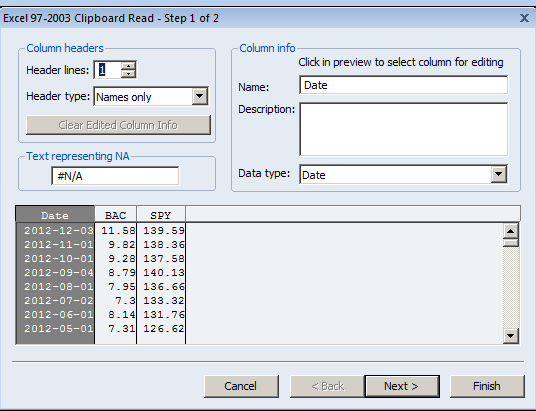
\includegraphics[height = 6cm]{Import}
\caption{Import data wizard}
\label{import}
\end{figure}

Most of the options should be clear. The main thing that you have to note is that the series that contains the information about the date should be specified.  One you have imported the data, you should have the following series: bac, spy and date.  You can delete the date series so long as the date has been specified correctly and the share price numbers line up alongside the correct month.

The Eviews workspace should look like Figure \ref{WP}.  The additionl series 'c' and 'resid' are always present.  They provide places for Eviews to put the estimated cofficients and the residuals. 

\begin{figure}[h!]
\graphicspath{{"../Eviews/Figures/"}}
\centering
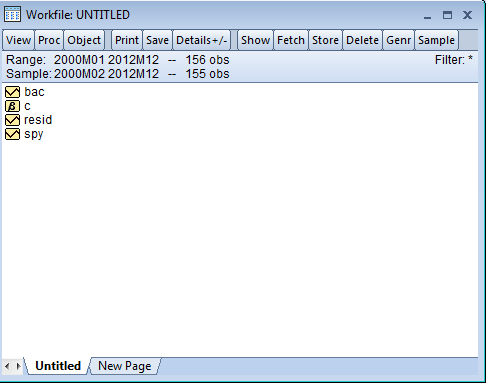
\includegraphics[height = 6cm]{Workspace}
\caption{Workspace with series added}
\label{WP}
\end{figure}

\section{Manipulating Series}
Once you have imported the raw data series into Eviews, it is possible to create new series by manipulating the existing numbers.  This can be done in one of three ways:  Using the command line, using "Quick" and then 'Series" from the menu or by creating a new "series" "Object".  We have used the command line at the top. 

To turn the raw share price data into returns it is necessary to calculate the percentage change in the share price each month. The special \verb  @pch  Eviews command will calculate the percentage change.  Figure \ref{RC} shows how this can be written in the command area.  The command 'series' will create a new series, the next element is the name (bacr in this case) and third term will specify the calculation. 

\begin{figure}[h!]
\graphicspath{{"../Eviews/Figures/"}}
\centering
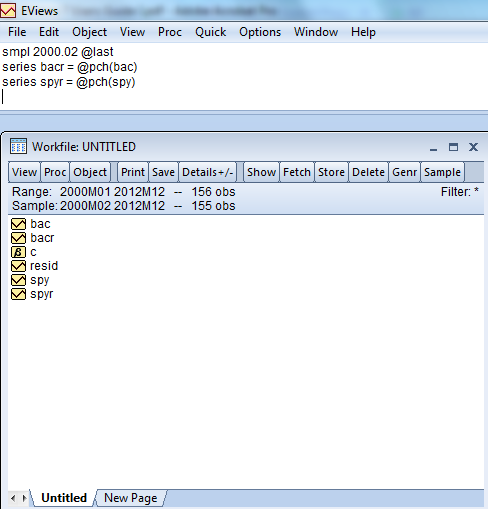
\includegraphics[height = 6cm]{Returncodefull}
\caption{Command line creation of return series}
\label{RC}
\end{figure}

\section{Estimating an equation}
Once the data have been imported and manipulated as needed the next step is to estimate the relationships between the variables.  Eviews will allow a number of different estimation techniques. However, we will use OLS.  This can be done by using the command 'equation' in the command line or 'quick-estimation' from the menu.  

Figure \ref{eq} shows the commands for OLS with the 'eq1.ls' the name of the equation and then the specification of the equation with the dependent variable followed by 'c' for the constant and then the explanatory variables.  In this case there is only one explanatory variable and that is 'spyr'. 

\begin{figure}[h!]
\graphicspath{{"../Eviews/Figures/"}}
\centering
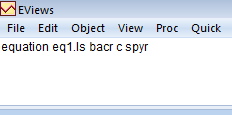
\includegraphics[height = 6cm]{equation}
\caption{Specifying the OLS equation}
\label{eq}
\end{figure}

The result of the estimation of Equation \ref{eq} is shown in Figure \ref{OLS}. The $R^2$ indicates the proportion of the change in the dependent variable that is explained by the model. In this case it is about 30\%. Some of the other figures that are presented here are explained below.    

\begin{figure}[h!]
\graphicspath{{"../Eviews/Figures/"}}
\centering
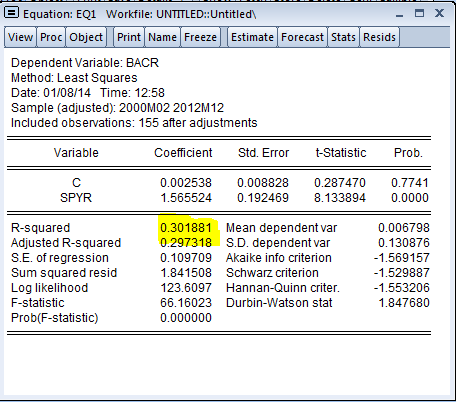
\includegraphics[height = 6cm]{eq1r2}
\caption{Estimated equation output: R squared}
\label{OLS}
\end{figure}



\section{Testing coefficients}
The relationship between the dependent and explanatory variables is estimated with some imprecision.  With a different sample a different estimate would be made.  We would like to know something about the range of possible estimates so that we can assess whether this estimated relationship is reliable.   

The estimated relationship between the return on Bank or America and the return on the S\&P 500 $(\beta_1)$ is a \emph{random variable} as it can take different values for different samples.  If it is assumed that the random variable has a \emph{normal distribution} and there are estimates of the mean and the standard deviation of this distribution, it will be possible to make inferences about the distribution of our estimated relationship. 

\begin{knitrout}
\definecolor{shadecolor}{rgb}{0.969, 0.969, 0.969}\color{fgcolor}\begin{figure}[]

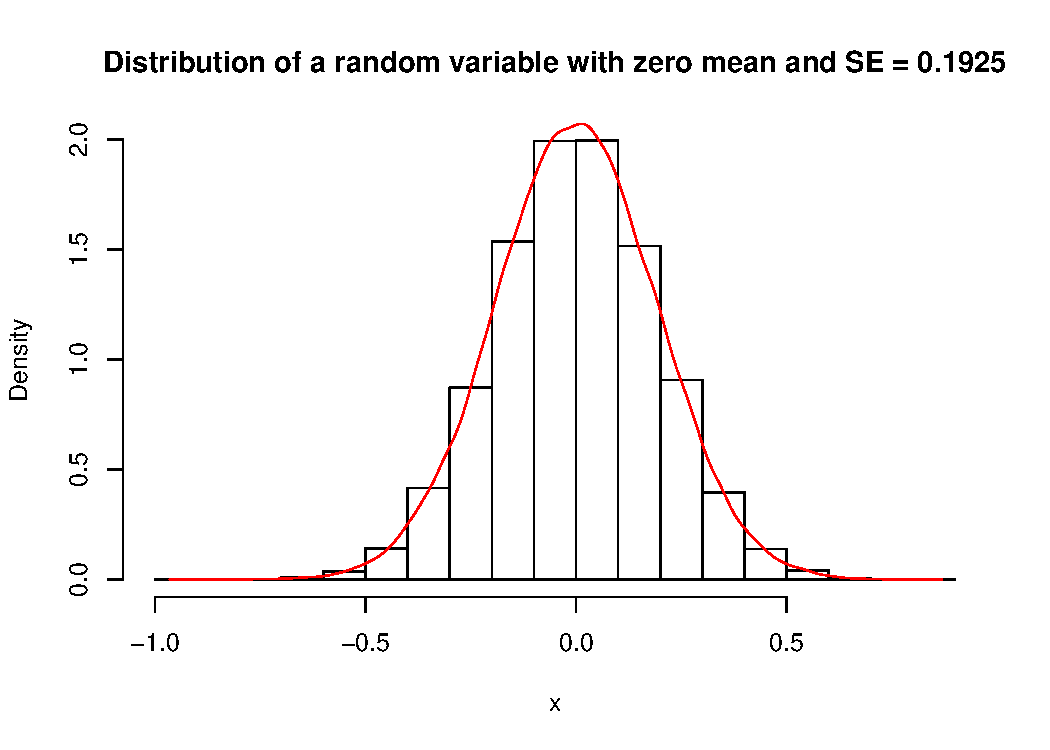
\includegraphics[width=\maxwidth]{figure/Normal} \caption[Normal Distribution]{Normal Distribution\label{fig:Normal}}
\end{figure}


\end{knitrout}


Figure \ref{fig:Normal} shows a normal distribution with a mean of zero and a standard error of 0.1925.  It is clear that an estimate in the region of 1.56 is very unlikely to be seen if the mean is actually zero.  This can be tested formally. 

\subsection{T-stats}
It can be shown that the estimate of $\beta_1$ is the best estimate of the mean of the random variable and the standard error is the estimated standard deviation of this estimate.  Therefore it is possible to construct \emph{t-statistics} to assess the likelihood that the estimated value of $\beta_1$ could be recorded under the null hypothesis that the true value of the relationship is zero. This will indicate how many standard errors the estimated value is from the hypothesised value.  If the t-stat is above or below two standard errors, it is an indication that the such an outcome would be extremely unlikely.  Indeed, if the random variable is distributed normally, this would only happen in 5 times out of 100 as 95\% of the reading would be within 2 standard errors of the mean.

\begin{align*}
\text{t-stat} =& \frac{\text{estimator} - \text{hypothesised value}}{\text{standard error of the estimator}}\\
\\[0.1cm]
%this will add the space
 =& \frac{\hat{\beta_1}-\beta_{1,0}}{SE(\hat{\beta_1})}
\end{align*}

The t-statistic is shown in Figure \ref{TS} where it is highlighted in yellow.  The calculation is $(1.56 - 0)/0.1925$. This shows that the estimate of 1.56 is more than 8 standard errors away from zero and therefore it is unlkely that this could have been seen if the reading was actually zero.  The final column 'Prob' gives the probability of seeing a value of 1.56 when the value is actually zero.  This is so small there is no reading.  At the conventional statistical level of 5\%, the null hypothesis that $\beta_0$ is zero is rejected.  

\begin{figure}[h!]
\graphicspath{{"../Eviews/Figures/"}}
\centering
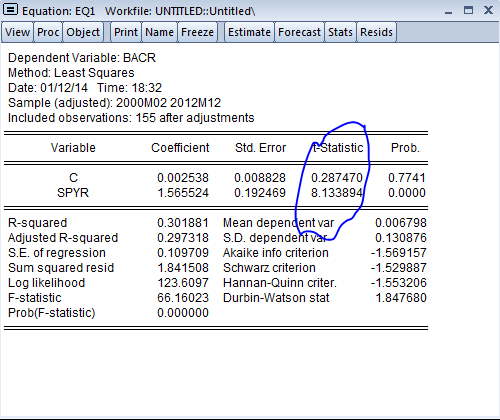
\includegraphics[height = 6cm]{tstat}
\caption{T-statistic}
\label{TS}
\end{figure}

By contrast, the estimate of $\beta_0$ is 0.0025 with a standard error of  0.0088.  The t-statistic here shows that this estimate is just 0.28 standard errors away from zero and that this could be seen with a probability of 77\%. The null hypothesis that $\beta_0$ is zero cannot be rejected. 


\end{document}
